\chapter{Application Layer}




\section{Principles of the Network Applications}

\subsection{Network Applicatoin Architectures}

\textbfit{Application Architecture} is designed by the application developer and \textit{dictates how the application is structured} over
various end systems.\\

Two predominant architectural paradigms:
\begin{enumerate}
    \item client-server architecture
    \item peer-to-peer(P2P) architecture
\end{enumerate}

\subsubsection{Client-Server}
\begin{enumerate}
    \item Server: the always-on host which services requests from many other hosts.
    \item Client: the end host whic request services from the server.
\end{enumerate}

Note that with the client-server architecture, clients do not directly communicate with each
other;for example, in the Web application, two browsers do not directly communi-
cate.\\
Another characteristic of the client-server architecture is that \textbfit{the server has a
    fixed, well-known address, called an IP address}. Because
the server has a fixed, well-known address, and because the server is always on, a
client can always contact the server by sending a packet to the server’s IP address.\\
Some well-known applications within client-server architecture:
\begin{enumerate}
    \item Web
    \item FTP
    \item Telnet
    \item e-mail
\end{enumerate}



\subsection{P2P architecture}

There is minimal (or no) reliance on dedicated servers in
data centers.Instead the application exploits direct communication between pairs of
intermittently connected hosts, called peers.\\

Characteristics that P2P architecture has:
\begin{enumerate}
    \item \textbfit{Self-Scalability}:although each peer generates
          workload by requesting files, each peer also adds service capacity to the system
          by distributing files to other peers.
    \item Cost effictive: normally don’t require significant server infrastructure and server bandwidth
\end{enumerate}

The problems that P2P need to face:
\begin{enumerate}
    \item ISP's asymmetrical bandwidth usage: ISPs are dimensioned for much more downstream than upstream traffic. But in p2p architecture, every residential ISPs will face a gigantic amount of upstream traffic.
    \item Security: Because of their highly distributed and open nature, P2P applications can be a challenge to secure.
    \item Incentives: Need users to volunteer bandwidth, storage, and computation resources to application.
\end{enumerate}

\subsection{Transport services available to applications}

We can broadly classify the possible services along four dimensions:
\begin{enumerate}
    \item Reliable data transfer
    \item Throughput
    \item Timing
    \item Security
\end{enumerate}




\section{Socket}

Most applications consist of pairs of communicating processes, with the two processes in each pair sending messages to each other.\\
\textbfit{Socket}: the interface that a process sends messages into, and receives messages from.

\begin{figure}[!h]
    \centering
    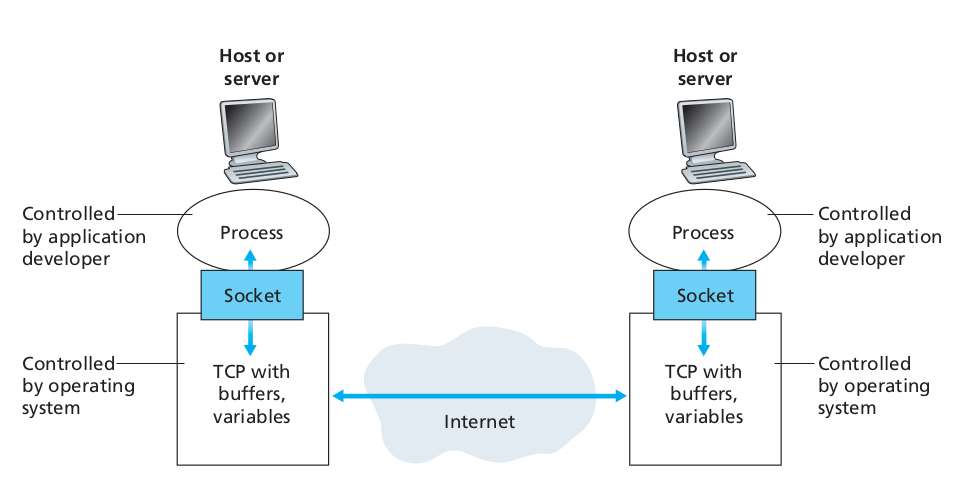
\includegraphics[width=0.7\textwidth]{chapters/chapter2/socket.png}
    \caption{Socket}
    \label{c2_socket}
\end{figure}

Socket is also referred as the API between the application and the network. The developer has control
of everything on the application-layer side but only little control of the transport-layer side of the socket:
\begin{enumerate}
    \item the choice of transport protocol
    \item fix a few transport-layer parameters such as maximum buffer and maximum segment sizes.
\end{enumerate}

\subsection{Address Processes}

Similarly, in order for a process running on one host to send packets to a
process running on another host, the receiving process needs to have an address.
In particular:
\begin{enumerate}
    \item The address of the host:\ \textbfit{IP address}.
    \item an identifier that specifies the receiving process in the destination host: \textbfit{Port number}.
\end{enumerate}

Some ports are reserved by well-known applications. For example, a Web server has port number 80. A mail server process has port number 25.



\section{The Web and HTTP}
The Web operates on demand.
\subsection{Overiew of HTTP}

The Web's application-layer protocol: HTTP(HyperText Transfer Protocol). HTTP is implemented both in client program and server program.
HTTP defines the structure of the messages and how the client and server exchange the messages.\\
\begin{center}
    Web browsers: Client side of HTTP.\\
    Web servers: Server side of HTTP, addressable by a URL.
\end{center}


\subsubsection{HTTP uses TCP}
The flow:
\begin{enumerate}
    \item The HTTP client initiates a TCP connection with the server.
    \item The HTTP client sends request messages into its socketnd and waits to receive HTTP response messages from its socket interface.
    \item The HTTP server receives request from its socket and sends response into its socket interface.
    \item The HTTP client receives the response.
\end{enumerate}

Another important thing is that HTTP is \tbi{stateless protocol}.


\subsection{HTTP with different connections}
There are two connection types for HTTP:
\begin{enumerate}
    \item Non-persistent connection: the application sends response using existing TCP connection.
    \item Persistent connection: the appication sends each response with a new TCP connection.
\end{enumerate}

\tbi{RTT(Round Trip Time)}

Non-persistent connection will take around two RTT for a single HTML file,and for each TCP established the TCP
variables need to be stored in both client and server side. This can place a significant burden on the Web server.\\

Persistent connection will only take one RTT once the connection is
established, and persistent connection with pipelining is the default mode of the HTTP.


\subsection{HTTP Request Format}
\begin{center}
    GET /somedir/page.html HTTP/1.1\\
    Host: www.someschool.edu\\
    Connection: close\\
    User-agent: Mozilla/5.0\\
    Accept-language: fr
    \label{c2_http_request}
\end{center}

The first line is called: the \tbi{request line};
The subsequent lines are called: the \tbi{header lines}.\\
The request line has three fields:
\begin{enumerate}
    \item The method field: including \tbi{GET,POST,HEAD,PUT} and \tbi{DELETE}.
    \item The URL field
    \item The HTTP version field
\end{enumerate}

The great majority of HTTP request messages use the GET method. The GET
method is used when the browser requests an object, with the requested object iden tified in the URL field.\\

The header line \tbi{Host: wwwwww.someschool.edu} specifies the host on which the object resides. The header line \tbi{Connection: close}
tells the server close the connection after sending the requested object. The \tbi{User-agent} and \tbi{Accept-Language} are self-explanatory.\\

\newpage

\begin{figure}[!h]
    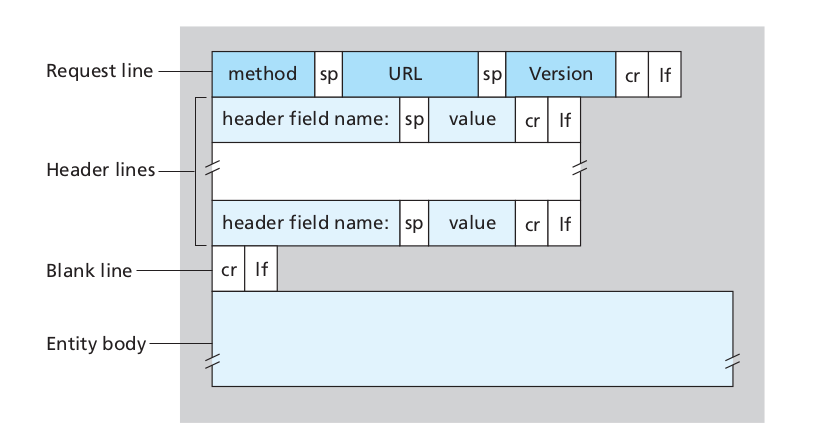
\includegraphics[width=0.95\textwidth]{chapters/chapter2/HTTP_Format.png}
    \caption{General format of an HTTP request message}
    \label{c2_http_format}
\end{figure}

The \tbi{entity body} is empty with \tbi{GET} method, but is used in \tbi{POST} method:HTTP client
often uses the POST method when the user fills out a form. For example, when a
user provides search words to a search engine. \\
However HTML forms often use the \tbi{GET} method and include the inputted data in the request URL. For example, inputted data is banana and money,
then the URL will look like \underlineit{www.somesite.com/search?monkeys\&bananas}.
The \tbi{HEAD} method only responds with an HTTP message but it leaves out the requested object(used to debug).\\
The \tbi{PUT} method allows a user to upload an object to specific path on specific Web server. It is also used by applications that need to
upload objects to Web servers.\\
The \tbi{DELETE} method allows a user, or an application, to delete an
object on a Web server.


\subsection{HTTP Reponse Format}




\begin{center}
    HTTP/1.1 200 OK\\
    Connection: close\\
    Date: Tue, 09 Aug 2011 15:44:04 GMT\\
    Server: Apache/2.2.3 (CentOS)\\
    Last-Modified: Tue, 09 Aug 2011 15:11:03 GMT\\
    Content-Length: 6821\\
    Content-Type: text/html\\
    (data data data data data ...)
\end{center}

The example has three sections: an initial \tbi{status line}, six \tbi{header line}, and then the \tbi{entity body}.\\
\subsubsection{The status line has three fields:}

\begin{enumerate}
    \item The protocol version field
    \item A status code: 200 in the example
    \item A corresponding status message.
\end{enumerate}

\subsubsection{The six header lines:}

\begin{enumerate}
    \item \tbi{Connection: close} header line: tell the client that it is going to close the TCP connection.
    \item The \tbi{Date:} header line indicates the time and date when the HTTP response was created and sent by the server.
    \item The \tbi{Server:} header line indicates that the message was generated by an Apache Web server.
    \item The \tbi{Last-Modified:} header line indicates the time and date when the object was created or last modified.
    \item The \tbi{Content-Length:} header line indicates the number of bytes in the object being sent.
    \item The \tbi{Content-Type:} header line indicates that the object in the entity body is HTML text.
\end{enumerate}


\subsubsection{General format of an HTTP response message}

\begin{figure}[!h]
    \centering
    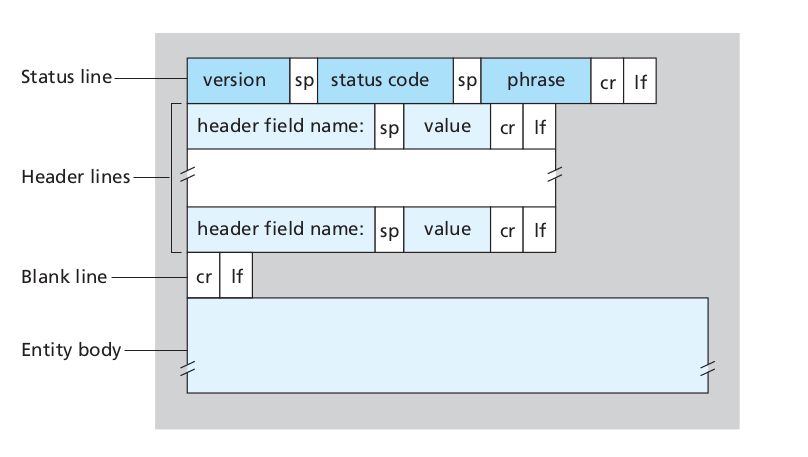
\includegraphics[width=0.9\textwidth]{chapters/chapter2/HTTP_Reponse_Message.png}
    \caption{General format of an HTTP response message}
    \label{c2_http_response}
\end{figure}

Some common status codes and associated phrases include:
\begin{enumerate}
    \item \tbi{200 OK}: Request succeeded and the information is returned in the response.
    \item \tbi{301 Moved Permanently}: Requested object has been permanently moved;
          the new URL is specified in Location: header of the response message. The
          client software will automatically retrieve the new URL.
    \item \tbi{400 Bad Request}: This is a generic error code indicating that the request
          could not be understood by the server.
    \item \tbi{404 Not Found}: The requested document does not exist on this server.
    \item \tbi{505 HTTP Version Not Supported}: The requested HTTP protocol
          version is not supported by the server.
\end{enumerate}


\subsection{Cookies}
HTTP use cookies to identify users.

\begin{figure}[!h]
    \centering
    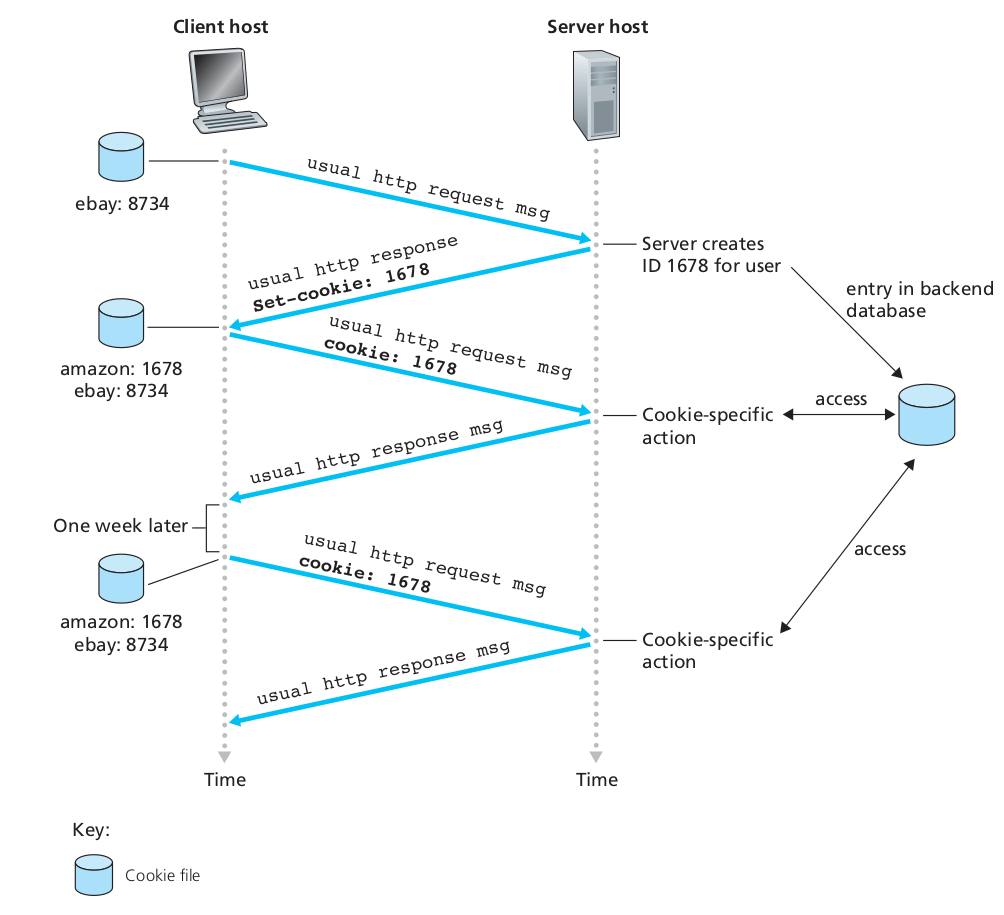
\includegraphics[width=0.9\textwidth]{chapters/chapter2/UserState_cookie.png}
    \caption{Use cookie to identify users}
    \label{c2_cookies}
\end{figure}

\subsubsection{Major cookies components}
\begin{enumerate}
    \item A cookie header line in the HTTP response message.
    \item A cookie header line in the HTTP request message.
    \item A cookie file kept on the user’s end system and managed by the
          user’s browser.
    \item A back-end database at the Web site.
\end{enumerate}

Flows of using cookies:
\begin{enumerate}
    \item Alice send HTTP request message without a cookie header line.
    \item The server generates a new cookies number and stores it to the database.Then repsonses with Set-cookie: header \tbi{Set-cookie: 1678}.
    \item When Alice receives the response message, her browsers appends a line to the special cookie file that it manages.
    \item In the following requests, Alice's browser will include the cookie for the server in the header lines. Like \tbi{Cookie: 1678}.
    \item The server will identify Alice with the cookie it receives in the header liens.
\end{enumerate}



\subsection{Web Caching}
A \tbi{Web cache}—also called a \tbi{proxy server}—is a network entity that satisfies HTTP
requests on the behalf of an origin Web server. \underlineit{The Web cache is both a client and a server}.

\begin{figure}
    \centering
    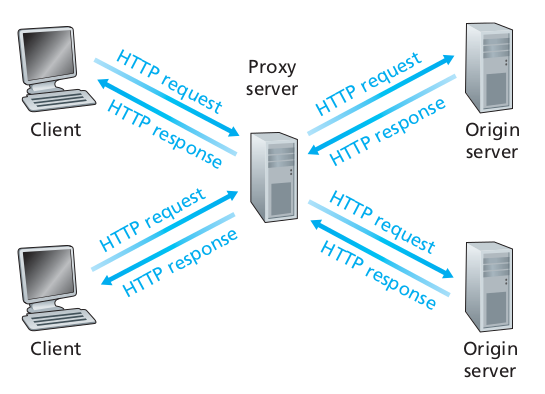
\includegraphics[width=0.6\textwidth]{chapters/chapter2/web_cache.png}
    \caption{Web Caching}
    \label{c2_web_caching}
\end{figure}

The web caching process:
\begin{enumerate}
    \item The browser establishes TCP connection to the Web cache and sends HTTP request for the object to the Web cache
    \item The Web cache checks to see if it has a copy of the object stored locally. If it
          does, the Web cache returns the object within an HTTP response message to
          the client browser.
    \item If the Web cache does not have a copy of the object, it sends HTTP request for the object to the origin server.
    \item The web cache receives the object from the origin server with HTTP response, it stores a copy of the object and sends back to the browser.
\end{enumerate}

Typically a Web cache is purchased and installed by an ISP. For example, a uni-
versity might install a cache on its campus network and configure all of the campus
browsers to point to the cache.Or a major residential ISP (such as AOL) might
install one or more caches in its network and preconfigure its shipped browsers to
point to the installed caches.\\

\subsubsection{Advantage of using a web cache/proxy server}

\begin{enumerate}
    \item A Web
          cache can substantially reduce the response time for a client request, particularly if the
          bottleneck bandwidth between the client and the origin server is much less than the bot-
          tleneck bandwidth between the client and the cache.
    \item Web caches can substantially reduce traffic on an institution’s access link to the Internet. By reducing traffic, the institution does not have to upgrade bandwidth as quickly, thereby
          reducing costs.
    \item Web caches can substantially reduce Web traffic in the Internet as a whole, thereby improving performance for all applications.
\end{enumerate}


\insertImage{width=0.4\textwidth}{chapters/chapter2/Cache_example.png}{Adding a cache to the institutional network}{c2_cache_example}

Suppose that the average object size is 1Mbits and that the average request rate from instution's
browsers to origin server is 15 requests per second.\\
The traffic intensity on the LAN is:
\begin{equation}
    (15 requests/sec) \cdot (1 Mbits/request) / (100Mps) = 0.15
    \label{c2_lan_traffic_intensity}
\end{equation}

The traffic intensity on the access link(from the Internet router to institution
router) is:
\begin{equation}
    (15 requests/sec) \cdot (1 Mbits/request) / (15Mps) = 1
    \label{c2_accessLink_traffic_intensity}
\end{equation}
Which is really bad and goes to infinite.

However, when we use the Web cache in the \autoref{c2_cache_example} when the hit rate is 0.4,
we will a traffic intensity on the access link:
\begin{equation}
    (15*0.6 requests/sec) \cdot (1 Mbits/request) / (15Mps) =0.6
\end{equation}
Which is much better.

\subsubsection{The conditional \textbf{GET}}


The Web cache uses \tbi{conditional GET} to check whether the copy of the object is up to date.
A HTTP request message is \tbi{conditional GET} if
\begin{enumerate}
    \item The request message uses the \tbi{GET} method.
    \item The request message includes an \tbi{If-Modified-Since:} header line.
\end{enumerate}

First, on the behalf of a requesting browser, a proxy cache sends a request message
to a Web server:

\begin{center}
    GET /fruit/banana HTTP/1.1\\
    HOST: www.walmart.ca
\end{center}

Second, the Web server receives the HTTP response from origin server:

\begin{center}
    HTTP/1.1 200 OK\\
    Date: Sat, 8 Oct 2011 15:39:32\\
    Server: Apache/1.3.0 (UNIX)\\
    Last-Modified: Wed, 7 Sep 2011 09:23:24\\
    Content-Type: image/gif\\
    (data data data data data ...)
\end{center}

The Web cache would forward the object to the requesting browser and store a copy of it.
When the next time someone sends a same request message, the Web cache would send a \tbi{conditional
    GET}:

\begin{center}
    GET /fruit/banana HTTP/1.1\\
    HOST: www.walmart.ca\\
    If-modified-since: Wed, 7 Sep 2011 09:23:24
\end{center}

Suppose the object is not updated after the last \tbi{GET}, the origin server would response:

\begin{center}
    HTTP/1.1 304 Not Modified\\
    Date: Sat, 15 Oct 2011 15:39:29\\
    Server: Apache/1.3.0 (Unix)\\
    (empty entity body)
\end{center}

\tbi{304 Not Modified} indicates that the requested object is not modified since Wed, 7 Sep 2011 09:23:24.
Therefore, it doesn't attach the data in the entity. The Web cache would forward the local copy of the
object back to the browser.\\

Note that an HTTP request/response message is ne